\documentclass[12pt,a4paper]{article}
\usepackage[utf8]{inputenc}
\usepackage[margin=1in]{geometry}
\usepackage{amsmath}
\usepackage{amssymb}
\usepackage{amsthm}
\usepackage{graphicx}
\usepackage{booktabs}
\usepackage{float}
\usepackage{hyperref}
\usepackage{xcolor}
\usepackage{listings}
\usepackage{tikz}
\usepackage{algorithm}
\usepackage{algpseudocode}

\usetikzlibrary{shapes.geometric, arrows, positioning, calc}

% Define colors
\definecolor{codebackground}{rgb}{0.95,0.95,0.95}
\definecolor{keywordcolor}{rgb}{0.0,0.0,0.5}
\definecolor{commentcolor}{rgb}{0.0,0.5,0.0}

% Listing style
\lstset{
    backgroundcolor=\color{codebackground},
    basicstyle=\ttfamily\small,
    keywordstyle=\color{keywordcolor}\bfseries,
    commentstyle=\color{commentcolor}\itshape,
    breaklines=true,
    frame=single,
    numbers=left,
    numberstyle=\tiny,
}

% Theorem environments
\newtheorem{definition}{Definition}[section]
\newtheorem{theorem}{Theorem}[section]
\newtheorem{example}{Example}[section]

\title{\textbf{Comprehensive Guide to Time Series Forecasting:\\Methods and Evaluation Strategies}}
\author{Payroll Forecasting System Documentation}
\date{\today}

\begin{document}

\maketitle

\begin{abstract}
This document provides a comprehensive guide to understanding the forecasting methodology implemented in the payroll prediction system. We detail seven distinct forecasting models (AR(1), AR(2), Ridge, Lasso, Pooled Fixed Effects, Unpooled, and XGBoost) and four evaluation strategies (Train/Validation/Test Split, Recursive Multi-Step Forecasting, Time Series Cross-Validation, and Nested Cross-Validation). Each method is explained with mathematical rigor, implementation details, and practical considerations. This guide serves as the definitive reference for understanding model selection, evaluation methodology, and error estimation in time series forecasting contexts.
\end{abstract}

\tableofcontents
\newpage

%==============================================================================
\section{Introduction}
%==============================================================================

\subsection{Problem Statement}

We address the problem of forecasting employee salaries (gross salary: \textit{salaire\_brut}) over a 6-month horizon. Given a panel dataset containing:
\begin{itemize}
    \item $N = 30$ employees
    \item $T = 24$ months of historical data per employee
    \item Target variable: $y_{it}$ representing the gross salary of employee $i$ at time $t$
\end{itemize}

The objective is to predict the last 6 months ($t = 19, 20, \ldots, 24$) for each employee, using the first 18 months for training and validation.

\subsection{Data Structure}

The data follows a \textbf{long format} panel structure:
\begin{equation}
\mathcal{D} = \{(i, t, y_{it}) : i \in \{1, \ldots, 30\}, t \in \{1, \ldots, 24\}\}
\end{equation}

Each observation is uniquely identified by the tuple $(i, t)$, and the dataset is sorted by employee ID and month.

\subsection{Evaluation Philosophy}

A critical distinction must be made between \textbf{optimistic} and \textbf{realistic} error estimation:

\begin{itemize}
    \item \textbf{Optimistic (One-Step-Ahead)}: Each prediction uses actual historical values as inputs
    \item \textbf{Realistic (Recursive Multi-Step)}: Predictions feed back as inputs, accumulating errors
\end{itemize}

This document extensively covers both approaches, highlighting the often dramatic differences in performance.

\subsection{Statistical Models vs. Machine Learning Models}

It is important to distinguish between \textbf{statistical models} and \textbf{machine learning (ML) models}, as both are used in this forecasting system.

\subsubsection{Statistical Models (AR, Ridge, Lasso, Pooled/Unpooled)}

Statistical models are characterized by:
\begin{itemize}
    \item \textbf{Explicit assumptions} about the data generation process (e.g., $y_t = \beta_0 + \beta_1 y_{t-1} + \epsilon_t$ where $\epsilon_t \sim \mathcal{N}(0, \sigma^2)$)
    \item \textbf{Parametric form}: The model structure is pre-specified with a finite number of interpretable parameters
    \item \textbf{Closed-form solutions}: Often solvable analytically (e.g., OLS: $\hat{\beta} = (X^TX)^{-1}X^Ty$)
    \item \textbf{Inference-focused}: Designed for hypothesis testing, confidence intervals, and understanding relationships
    \item \textbf{Interpretability}: Parameters have clear meanings (e.g., $\beta_1$ = effect of lag-1 on current value)
    \item \textbf{Theory-driven}: Based on established statistical theory (e.g., time series econometrics)
\end{itemize}

\textbf{Examples in this work:} AR(1), AR(2), Ridge Regression, Lasso, Pooled Fixed Effects, Unpooled Models

\subsubsection{Machine Learning Models (XGBoost)}

Machine learning models are characterized by:
\begin{itemize}
    \item \textbf{Minimal assumptions}: Let the data reveal patterns without imposing strict distributional assumptions
    \item \textbf{Non-parametric or high-dimensional}: Flexible model structure that adapts to data complexity
    \item \textbf{Iterative optimization}: Trained through algorithms (gradient descent, boosting) rather than closed-form solutions
    \item \textbf{Prediction-focused}: Optimized primarily for predictive accuracy rather than parameter interpretation
    \item \textbf{Black-box nature}: Internal mechanics may be opaque (e.g., ensemble of 100 trees is hard to interpret)
    \item \textbf{Data-driven}: Performance improves with large datasets; learns complex non-linear patterns automatically
\end{itemize}

\textbf{Examples in this work:} XGBoost (Gradient Boosting with decision trees)

\subsubsection{Hybrid Approaches}

Note that Ridge and Lasso regression occupy a middle ground:
\begin{itemize}
    \item They are \textbf{statistical models} at their core (linear regression with explicit assumptions)
    \item But they incorporate \textbf{ML-style regularization} (penalizing model complexity to prevent overfitting)
    \item They require hyperparameter tuning ($\alpha$) like ML models
    \item They maintain interpretability while using optimization techniques from ML
\end{itemize}

\subsubsection{Why This Matters for Forecasting}

\begin{table}[H]
\centering
\small
\begin{tabular}{lcc}
\toprule
\textbf{Criterion} & \textbf{Statistical (AR)} & \textbf{ML (XGBoost)} \\
\midrule
Model complexity & Low (3 parameters) & High (100 trees, thousands of splits) \\
Interpretability & High & Low \\
Assumption requirements & Strict & Minimal \\
Training data needed & Moderate & Large \\
Handles non-linearity & No & Yes \\
Error accumulation & Severe (+159\%) & Minimal (-8\%) \\
Production complexity & Simple & Moderate \\
\bottomrule
\end{tabular}
\caption{Statistical vs. ML models for time series forecasting}
\end{table}

The key finding in this work is that the \textbf{ML approach (XGBoost) is more robust} to recursive forecasting errors, likely because its ensemble nature and non-linear capabilities allow it to learn more stable prediction patterns.

%==============================================================================
\section{Mathematical Notation and Preliminaries}
%==============================================================================

\subsection{Core Notation}

\begin{table}[H]
\centering
\begin{tabular}{cl}
\toprule
\textbf{Symbol} & \textbf{Description} \\
\midrule
$y_{it}$ & Gross salary of employee $i$ at time $t$ \\
$\hat{y}_{it}$ & Predicted salary of employee $i$ at time $t$ \\
$N$ & Number of employees (30) \\
$T$ & Total time periods (24 months) \\
$T_{train}$ & Training period length (typically 15 months) \\
$T_{val}$ & Validation period length (3 months) \\
$T_{test}$ & Test period length (6 months) \\
$p$ & Number of lags in autoregressive models \\
$\alpha$ & Regularization parameter (Ridge/Lasso) \\
\bottomrule
\end{tabular}
\caption{Core mathematical notation}
\end{table}

\subsection{Performance Metrics}

All models are evaluated using the following metrics:

\subsubsection{Root Mean Squared Error (RMSE)}
\begin{equation}
\text{RMSE} = \sqrt{\frac{1}{n}\sum_{i=1}^{n}(y_i - \hat{y}_i)^2}
\end{equation}

\textbf{Important: Pooled vs. Per-Employee Aggregation}

In panel data forecasting, RMSE can be computed in two ways:

\textbf{Method 1: Pooled RMSE (Used in this document)}
\begin{equation}
\text{RMSE}_{\text{pooled}} = \sqrt{\frac{1}{N \times T_{test}}\sum_{i=1}^{N}\sum_{t=1}^{T_{test}}(y_{it} - \hat{y}_{it})^2}
\end{equation}

where $n = N \times T_{test}$ is the total number of predictions across all employees.

\textbf{Method 2: Per-Employee Average}
\begin{equation}
\text{RMSE}_{\text{avg}} = \frac{1}{N}\sum_{i=1}^{N}\sqrt{\frac{1}{T_{test}}\sum_{t=1}^{T_{test}}(y_{it} - \hat{y}_{it})^2}
\end{equation}

This computes RMSE for each employee separately, then averages.

\textbf{Why We Use Pooled RMSE:}
\begin{itemize}
    \item \textbf{Standard ML practice}: All major libraries (sklearn, TensorFlow, PyTorch) use pooled metrics by default
    \item \textbf{Total accuracy}: Reflects performance on ALL predictions, not average employee
    \item \textbf{Equal weighting}: Each prediction weighted equally (each salary forecast equally important)
    \item \textbf{Unbiased estimation}: Pooled RMSE is the unbiased estimator of population prediction error
    \item \textbf{Comparability}: Enables direct comparison with published research using standard metrics
\end{itemize}

\textbf{Note:} Per-employee averaging typically yields lower values (e.g., 90 vs. 145 in our data) because it weights employees equally regardless of prediction difficulty or error magnitude. Pooled RMSE correctly reflects total system accuracy.

\subsubsection{Normalized Root Mean Squared Error (NRMSE)}
\begin{equation}
\text{NRMSE} = \frac{\text{RMSE}}{\bar{y}} = \frac{\sqrt{\frac{1}{n}\sum_{i=1}^{n}(y_i - \hat{y}_i)^2}}{\frac{1}{n}\sum_{i=1}^{n}y_i}
\end{equation}

The NRMSE is our \textbf{primary metric} as it provides scale-independent comparison across employees and time periods.

\subsubsection{Mean Absolute Error (MAE)}
\begin{equation}
\text{MAE} = \frac{1}{n}\sum_{i=1}^{n}|y_i - \hat{y}_i|
\end{equation}

\subsubsection{Coefficient of Determination ($R^2$)}
\begin{equation}
R^2 = 1 - \frac{\sum_{i=1}^{n}(y_i - \hat{y}_i)^2}{\sum_{i=1}^{n}(y_i - \bar{y})^2}
\end{equation}

Note: In time series cross-validation, $R^2$ can be negative, indicating that the model performs worse than a naive mean predictor.

%==============================================================================
\section{Forecasting Models: Detailed Descriptions}
%==============================================================================

\subsection{Autoregressive Models (AR)}

\subsubsection{AR(1) Model}

\begin{definition}[AR(1) Model]
An autoregressive model of order 1 predicts the current value as a linear function of the previous value plus a time trend:
\begin{equation}
y_{it} = \beta_0 + \beta_1 \cdot y_{i,t-1} + \beta_2 \cdot t + \epsilon_{it}
\end{equation}
where:
\begin{itemize}
    \item $\beta_0$ is the intercept
    \item $\beta_1$ is the coefficient for the lag-1 term
    \item $\beta_2$ is the coefficient for the time trend
    \item $t$ is the time index
    \item $\epsilon_{it}$ is the error term
\end{itemize}
\end{definition}

\textbf{Feature Construction:}
\begin{enumerate}
    \item Create lag-1 feature: $x_{1,it} = y_{i,t-1}$
    \item Create time index: $x_{2,it} = t$
    \item Remove first observation (where lag is undefined)
\end{enumerate}

\textbf{Estimation:}
Ordinary Least Squares (OLS) regression:
\begin{equation}
\hat{\boldsymbol{\beta}} = (\mathbf{X}^T\mathbf{X})^{-1}\mathbf{X}^T\mathbf{y}
\end{equation}

\textbf{One-Step-Ahead Prediction:}
\begin{equation}
\hat{y}_{i,t} = \hat{\beta}_0 + \hat{\beta}_1 \cdot y_{i,t-1} + \hat{\beta}_2 \cdot t
\end{equation}

\textbf{Recursive Multi-Step Prediction:}
\begin{align}
\hat{y}_{i,t+1} &= \hat{\beta}_0 + \hat{\beta}_1 \cdot y_{i,t} + \hat{\beta}_2 \cdot (t+1) \\
\hat{y}_{i,t+2} &= \hat{\beta}_0 + \hat{\beta}_1 \cdot \hat{y}_{i,t+1} + \hat{\beta}_2 \cdot (t+2) \\
\hat{y}_{i,t+h} &= \hat{\beta}_0 + \hat{\beta}_1 \cdot \hat{y}_{i,t+h-1} + \hat{\beta}_2 \cdot (t+h)
\end{align}

Note the critical difference: in recursive forecasting, we use $\hat{y}_{i,t+h-1}$ (prediction) instead of $y_{i,t+h-1}$ (actual value).

\textbf{Recursive Prediction Algorithm:}

\begin{algorithm}[H]
\caption{AR(1) Recursive Multi-Step Forecasting}
\begin{algorithmic}[1]
\State \textbf{Input:} Trained model $(\hat{\beta}_0, \hat{\beta}_1, \hat{\beta}_2)$
\State \textbf{Input:} Last actual value $y_{i,t}$
\State \textbf{Input:} Forecast horizon $h = 6$
\State Initialize: $prev\_value \gets y_{i,t}$
\For{$s = 1$ to $h$}
    \State $\hat{y}_{i,t+s} \gets \hat{\beta}_0 + \hat{\beta}_1 \cdot prev\_value + \hat{\beta}_2 \cdot (t+s)$
    \State $prev\_value \gets \hat{y}_{i,t+s}$ \Comment{Use prediction for next step}
\EndFor
\State \textbf{Return:} $[\hat{y}_{i,t+1}, \hat{y}_{i,t+2}, \ldots, \hat{y}_{i,t+h}]$
\end{algorithmic}
\end{algorithm}

\subsubsection{AR(2) Model}

\begin{definition}[AR(2) Model]
An autoregressive model of order 2 uses the previous two values:
\begin{equation}
y_{it} = \beta_0 + \beta_1 \cdot y_{i,t-1} + \beta_2 \cdot y_{i,t-2} + \beta_3 \cdot t + \epsilon_{it}
\end{equation}
\end{definition}

\textbf{Feature Matrix:}
\begin{equation}
\mathbf{X}_i = \begin{bmatrix}
y_{i,2} & y_{i,1} & 3 \\
y_{i,3} & y_{i,2} & 4 \\
\vdots & \vdots & \vdots \\
y_{i,T-1} & y_{i,T-2} & T
\end{bmatrix}
\end{equation}

\textbf{Recursive Prediction Algorithm:}

\begin{algorithm}[H]
\caption{AR(2) Recursive Multi-Step Forecasting}
\begin{algorithmic}[1]
\State \textbf{Input:} Trained model $(\hat{\beta}_0, \hat{\beta}_1, \hat{\beta}_2, \hat{\beta}_3)$
\State \textbf{Input:} Last two actual values $(y_{i,t-1}, y_{i,t-2})$
\State \textbf{Input:} Forecast horizon $h = 6$
\State Initialize: $history \gets [y_{i,t-2}, y_{i,t-1}]$
\For{$s = 1$ to $h$}
    \State $\hat{y}_{i,t+s} \gets \hat{\beta}_0 + \hat{\beta}_1 \cdot history[1] + \hat{\beta}_2 \cdot history[0] + \hat{\beta}_3 \cdot (t+s)$
    \State Append $\hat{y}_{i,t+s}$ to $history$
    \State Remove first element from $history$ \Comment{Keep window size = 2}
\EndFor
\State \textbf{Return:} $[\hat{y}_{i,t+1}, \hat{y}_{i,t+2}, \ldots, \hat{y}_{i,t+h}]$
\end{algorithmic}
\end{algorithm}

\textbf{Error Accumulation:}
The AR(2) model is particularly susceptible to error accumulation because:
\begin{itemize}
    \item Each prediction depends on \textit{two} previous predictions (second-order recurrence)
    \item AR(1) has first-order error propagation: $e_{t+1} \approx \beta_1 e_t + \epsilon_{t+1}$ (depends on one past error)
    \item AR(2) has second-order error propagation: $e_{t+1} \approx \beta_1 e_t + \beta_2 e_{t-1} + \epsilon_{t+1}$ (depends on two past errors)
    \item More error dependencies create more severe compounding
    \item Empirical results show +159.5\% error increase (AR(2) recursive vs one-step) compared to +44.2\% for AR(1)
\end{itemize}

%==============================================================================
\subsection{Regularized Linear Models}

\subsubsection{Ridge Regression}

\begin{definition}[Ridge Regression]
Ridge regression adds an L2 penalty to the ordinary least squares objective:
\begin{equation}
\min_{\boldsymbol{\beta}} \left\{ \sum_{i=1}^{n}(y_i - \mathbf{x}_i^T\boldsymbol{\beta})^2 + \alpha \sum_{j=1}^{p}\beta_j^2 \right\}
\end{equation}
where $\alpha > 0$ is the regularization parameter.
\end{definition}

\textbf{Features Used:}
\begin{itemize}
    \item Time index: $t$
    \item Lag-1: $y_{i,t-1}$
    \item Lag-2: $y_{i,t-2}$
    \item Lag-3: $y_{i,t-3}$
\end{itemize}

\textbf{Closed-Form Solution:}
\begin{equation}
\hat{\boldsymbol{\beta}} = (\mathbf{X}^T\mathbf{X} + \alpha\mathbf{I})^{-1}\mathbf{X}^T\mathbf{y}
\end{equation}

\textbf{Hyperparameter Tuning:}
The regularization parameter $\alpha$ is selected from the grid:
\begin{equation}
\alpha \in \{0.1, 1.0, 10.0, 100.0\}
\end{equation}
using validation set performance (NRMSE).

\textbf{Feature Scaling:}
Ridge regression requires standardized features:
\begin{equation}
\tilde{x}_j = \frac{x_j - \mu_j}{\sigma_j}
\end{equation}
where $\mu_j$ and $\sigma_j$ are computed on the training set only.

\textbf{Recursive Forecasting with Ridge:}

\begin{algorithm}[H]
\caption{Ridge Recursive Multi-Step Forecasting}
\begin{algorithmic}[1]
\State \textbf{Input:} Trained Ridge model with scaler
\State \textbf{Input:} Last 3 actual values $[y_{i,t-3}, y_{i,t-2}, y_{i,t-1}]$
\State Initialize: $history \gets [y_{i,t-3}, y_{i,t-2}, y_{i,t-1}]$
\For{$s = 1$ to $6$}
    \State Construct feature vector: $\mathbf{x} = [t+s, history[2], history[1], history[0]]$
    \State Scale features: $\tilde{\mathbf{x}} = \text{scaler.transform}(\mathbf{x})$
    \State $\hat{y}_{i,t+s} \gets \text{model.predict}(\tilde{\mathbf{x}})$
    \State Append $\hat{y}_{i,t+s}$ to $history$
    \State Remove first element from $history$
\EndFor
\State \textbf{Return:} Predictions
\end{algorithmic}
\end{algorithm}

\subsubsection{Lasso Regression}

\begin{definition}[Lasso Regression]
Lasso uses L1 regularization for feature selection:
\begin{equation}
\min_{\boldsymbol{\beta}} \left\{ \sum_{i=1}^{n}(y_i - \mathbf{x}_i^T\boldsymbol{\beta})^2 + \alpha \sum_{j=1}^{p}|\beta_j| \right\}
\end{equation}
\end{definition}

\textbf{Key Differences from Ridge:}
\begin{itemize}
    \item L1 penalty promotes \textbf{sparsity} (some $\beta_j = 0$ exactly)
    \item No closed-form solution; requires iterative optimization
    \item Can perform automatic feature selection
    \item Same hyperparameter grid as Ridge
\end{itemize}

\textbf{Recursive Forecasting:}
Identical to Ridge (Algorithm 2), but using Lasso coefficients.

%==============================================================================
\subsection{Panel Data Models}

\subsubsection{Pooled Fixed Effects Model}

\begin{definition}[Pooled Fixed Effects]
The pooled model assumes a common time trend with employee-specific intercepts:
\begin{equation}
y_{it} = \alpha_i + \beta \cdot t + \epsilon_{it}
\end{equation}
where:
\begin{itemize}
    \item $\alpha_i$ is the fixed effect for employee $i$
    \item $\beta$ is the common time trend coefficient
\end{itemize}
\end{definition}

\textbf{Implementation via Dummy Variables:}
\begin{equation}
y_{it} = \sum_{j=1}^{N}\alpha_j \cdot \mathbb{1}(i=j) + \beta \cdot t + \epsilon_{it}
\end{equation}

\textbf{Matrix Form:}
\begin{equation}
\mathbf{y} = \mathbf{D}\boldsymbol{\alpha} + \mathbf{t}\beta + \boldsymbol{\epsilon}
\end{equation}
where $\mathbf{D}$ is the $(NT \times N)$ dummy matrix.

\textbf{Estimation:}
Standard OLS on augmented feature matrix:
\begin{equation}
\mathbf{X} = [\mathbf{D} \mid \mathbf{t}]
\end{equation}

\textbf{Prediction:}
For employee $i$ at time $t$:
\begin{equation}
\hat{y}_{it} = \hat{\alpha}_i + \hat{\beta} \cdot t
\end{equation}

\textbf{Note on Recursive Forecasting:}
Since the model depends only on time (not lagged values), one-step and recursive predictions are \textbf{identical}.

\subsubsection{Unpooled Model}

\begin{definition}[Unpooled Model]
Fit separate linear regression for each employee:
\begin{equation}
y_{it} = \alpha_i + \beta_i \cdot t + \epsilon_{it}
\end{equation}
where both intercept and slope are employee-specific.
\end{definition}

\textbf{Implementation:}
\begin{enumerate}
    \item For each employee $i$:
    \begin{equation}
    \hat{\beta}_i = \arg\min_{\beta} \sum_{t=1}^{T}(y_{it} - \alpha - \beta \cdot t)^2
    \end{equation}
    \item Store $N$ separate models
\end{enumerate}

\textbf{Advantages:}
\begin{itemize}
    \item Captures heterogeneous time trends
    \item No pooling bias
\end{itemize}

\textbf{Disadvantages:}
\begin{itemize}
    \item $2N$ parameters to estimate
    \item No information sharing across employees
    \item Poor performance with limited data
\end{itemize}

%==============================================================================
\subsection{Machine Learning: XGBoost}

\subsubsection{Model Description}

\begin{definition}[XGBoost]
XGBoost (eXtreme Gradient Boosting) is an ensemble of decision trees trained sequentially. Each tree corrects the errors of the previous ensemble:
\begin{equation}
\hat{y}^{(m)} = \hat{y}^{(m-1)} + \eta \cdot f_m(\mathbf{x})
\end{equation}
where:
\begin{itemize}
    \item $\hat{y}^{(m)}$ is prediction after $m$ trees
    \item $\eta$ is the learning rate
    \item $f_m$ is the $m$-th decision tree
\end{itemize}
\end{definition}

\textbf{Objective Function:}
\begin{equation}
\mathcal{L}^{(m)} = \sum_{i=1}^{n}l(y_i, \hat{y}_i^{(m)}) + \sum_{k=1}^{m}\Omega(f_k)
\end{equation}
where:
\begin{itemize}
    \item $l(\cdot)$ is the loss function (MSE for regression)
    \item $\Omega(f_k) = \gamma T + \frac{1}{2}\lambda \|\mathbf{w}\|^2$ is the regularization term
    \item $T$ is the number of leaves
    \item $\mathbf{w}$ are the leaf weights
\end{itemize}

\subsubsection{Feature Engineering for XGBoost}

\textbf{Lag Features:}
\begin{align}
x_{1,it} &= y_{i,t-1} \quad \text{(lag-1)} \\
x_{2,it} &= y_{i,t-2} \quad \text{(lag-2)} \\
x_{3,it} &= y_{i,t-3} \quad \text{(lag-3)}
\end{align}

\textbf{Rolling Statistics:}
\begin{align}
x_{4,it} &= \frac{1}{3}\sum_{j=1}^{3}y_{i,t-j} \quad \text{(3-month rolling mean)} \\
x_{5,it} &= \sqrt{\frac{1}{3}\sum_{j=1}^{3}(y_{i,t-j} - x_{4,it})^2} \quad \text{(3-month rolling std)}
\end{align}

\textbf{Time Index:}
\begin{equation}
x_{6,it} = t
\end{equation}

\textbf{Feature Matrix:}
\begin{equation}
\mathbf{X}_{it} = [x_{1,it}, x_{2,it}, x_{3,it}, x_{4,it}, x_{5,it}, x_{6,it}]^T
\end{equation}

\subsubsection{Hyperparameters}

\begin{table}[H]
\centering
\begin{tabular}{ll}
\toprule
\textbf{Parameter} & \textbf{Value} \\
\midrule
n\_estimators & 100 \\
learning\_rate & 0.1 \\
max\_depth & 3 \\
random\_state & 42 \\
\bottomrule
\end{tabular}
\caption{XGBoost hyperparameters}
\end{table}

\subsubsection{Recursive Forecasting with XGBoost}

\begin{algorithm}[H]
\caption{XGBoost Recursive Multi-Step Forecasting}
\begin{algorithmic}[1]
\State \textbf{Input:} Trained XGBoost model
\State \textbf{Input:} Historical values $[y_{i,1}, \ldots, y_{i,t}]$
\State Initialize: $history \gets [y_{i,t-2}, y_{i,t-1}, y_{i,t}]$
\For{$s = 1$ to $6$}
    \State $lag_1 \gets history[2]$
    \State $lag_2 \gets history[1]$
    \State $lag_3 \gets history[0]$
    \State $rolling\_mean \gets \frac{1}{3}(lag_1 + lag_2 + lag_3)$
    \State $rolling\_std \gets \sqrt{\frac{1}{3}\sum_{j}(history[j] - rolling\_mean)^2}$
    \State $time\_index \gets t + s$
    \State Construct: $\mathbf{x} = [lag_1, lag_2, lag_3, rolling\_mean, rolling\_std, time\_index]$
    \State Scale: $\tilde{\mathbf{x}} = \text{scaler.transform}(\mathbf{x})$
    \State $\hat{y}_{i,t+s} \gets \text{model.predict}(\tilde{\mathbf{x}})$
    \State Append $\hat{y}_{i,t+s}$ to $history$
    \State Remove first element from $history$
\EndFor
\State \textbf{Return:} Predictions
\end{algorithmic}
\end{algorithm}

\textbf{Key Observation:}
XGBoost shows \textbf{improved} performance with recursive forecasting (-8.4\% error change), making it uniquely robust among all tested models.

%==============================================================================
\section{Evaluation Methodologies}
%==============================================================================

\subsection{Method 1: Train/Validation/Test Split}

\subsubsection{Overview}

The traditional hold-out approach divides the time series into three consecutive segments.

\begin{figure}[H]
\centering
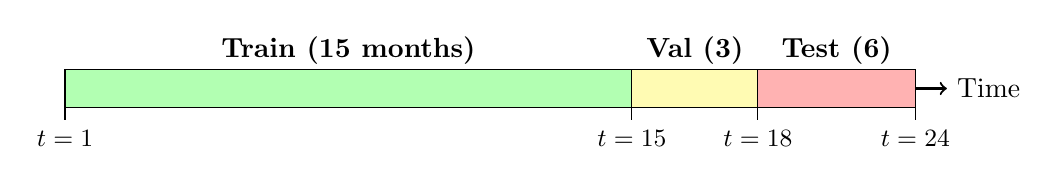
\begin{tikzpicture}[scale=0.8]
    % Timeline
    \draw[thick, ->] (0,0) -- (14,0) node[right] {Time};
    
    % Train
    \draw[fill=green!30] (0,-0.3) rectangle (9,0.3);
    \node at (4.5, 0.6) {\textbf{Train (15 months)}};
    
    % Validation
    \draw[fill=yellow!30] (9,-0.3) rectangle (11,0.3);
    \node at (10, 0.6) {\textbf{Val (3)}};
    
    % Test
    \draw[fill=red!30] (11,-0.3) rectangle (13.5,0.3);
    \node at (12.25, 0.6) {\textbf{Test (6)}};
    
    % Time labels
    \foreach \x/\label in {0/1, 9/15, 11/18, 13.5/24} {
        \draw (\x, -0.3) -- (\x, -0.5);
        \node at (\x, -0.8) {\small $t=\label$};
    }
\end{tikzpicture}
\caption{Train/Validation/Test split for time series}
\end{figure}

\subsubsection{Detailed Procedure}

\begin{algorithm}[H]
\caption{Train/Validation/Test Evaluation}
\begin{algorithmic}[1]
\State \textbf{Input:} Time series $\{y_{it}\}_{t=1}^{24}$ for each employee $i$
\State Set $T_{train} = 15$, $T_{val} = 3$, $T_{test} = 6$
\For{each employee $i$}
    \State Split data:
    \State \quad $\mathcal{D}_{train} = \{y_{it}\}_{t=1}^{15}$
    \State \quad $\mathcal{D}_{val} = \{y_{it}\}_{t=16}^{18}$
    \State \quad $\mathcal{D}_{test} = \{y_{it}\}_{t=19}^{24}$
    \State 
    \If{model has hyperparameters}
        \State Tune hyperparameters using $\mathcal{D}_{val}$
    \EndIf
    \State
    \State Retrain on $\mathcal{D}_{train} \cup \mathcal{D}_{val}$
    \State Predict on $\mathcal{D}_{test}$: $\{\hat{y}_{it}\}_{t=19}^{24}$
\EndFor
\State
\State \textcolor{blue}{\# Aggregate predictions (pooled approach)}
\State Initialize: $all\_y\_true = []$, $all\_y\_pred = []$
\For{each employee $i$}
    \State Append $y_{test}^{(i)}$ to $all\_y\_true$
    \State Append $\hat{y}_{test}^{(i)}$ to $all\_y\_pred$
\EndFor
\State
\State Compute pooled metrics on combined predictions:
\State \quad $\text{RMSE} = \sqrt{\frac{1}{n}\sum(all\_y\_true - all\_y\_pred)^2}$ where $n = N \times T_{test}$
\State \quad $\text{NRMSE} = \text{RMSE} / \text{mean}(all\_y\_true)$
\State \quad $\text{MAE}, R^2$ computed similarly on pooled data
\end{algorithmic}
\end{algorithm}

\subsubsection{One-Step-Ahead Prediction Strategy}

\textbf{Critical Detail:} In this method, each test prediction uses \textbf{actual} lagged values:

\begin{align}
\hat{y}_{i,19} &= f(y_{i,18}, y_{i,17}, y_{i,16}, \ldots) \quad \text{(uses actual $y_{i,18}$)} \\
\hat{y}_{i,20} &= f(y_{i,19}, y_{i,18}, y_{i,17}, \ldots) \quad \text{(uses actual $y_{i,19}$)} \\
\hat{y}_{i,21} &= f(y_{i,20}, y_{i,19}, y_{i,18}, \ldots) \quad \text{(uses actual $y_{i,20}$)}
\end{align}

This is \textbf{optimistic} because in real deployment, we would not have access to $y_{i,20}$ when forecasting $\hat{y}_{i,21}$.

\subsubsection{Advantages and Disadvantages}

\textbf{Advantages:}
\begin{itemize}
    \item Simple and interpretable
    \item Standard practice in machine learning
    \item Validation set allows hyperparameter tuning
    \item Provides best-case performance estimate
\end{itemize}

\textbf{Disadvantages:}
\begin{itemize}
    \item \textbf{Overestimates} real-world performance
    \item Single test period reduces reliability
    \item Ignores error accumulation
    \item Not suitable for production error estimation
\end{itemize}

%==============================================================================
\subsection{Method 2: Recursive Multi-Step Forecasting}

\subsubsection{Overview}

This method provides a \textbf{realistic} assessment by simulating actual deployment conditions where predictions feed back as inputs.

\subsubsection{Detailed Procedure}

\begin{algorithm}[H]
\caption{Recursive Multi-Step Evaluation}
\begin{algorithmic}[1]
\State \textbf{Input:} Trained model, last known values before test period
\State Set forecast horizon $h = 6$
\For{each employee $i$}
    \State Initialize: $history \gets \{y_{i,t}\}_{t=T_{train}+T_{val}-p}^{T_{train}+T_{val}}$
    \For{$s = 1$ to $h$}
        \State Construct features using $history$ (predictions, not actuals)
        \State $\hat{y}_{i,T_{train}+T_{val}+s} \gets f(history)$
        \State Update: $history \gets history \cup \{\hat{y}_{i,T_{train}+T_{val}+s}\}$
        \State Remove oldest value from $history$ to maintain window size
    \EndFor
\EndFor
\State
\State Compare $\{\hat{y}_{it}\}$ to $\{y_{it}\}$ for $t \in [19, 24]$
\State Compute metrics
\end{algorithmic}
\end{algorithm}

\subsubsection{Mathematical Formulation}

For an AR(2) model, the recursive prediction is:

\begin{align}
\hat{y}_{i,19} &= \hat{\beta}_0 + \hat{\beta}_1 y_{i,18} + \hat{\beta}_2 y_{i,17} + \hat{\beta}_3 \cdot 19 \\
\hat{y}_{i,20} &= \hat{\beta}_0 + \hat{\beta}_1 \hat{y}_{i,19} + \hat{\beta}_2 y_{i,18} + \hat{\beta}_3 \cdot 20 \\
\hat{y}_{i,21} &= \hat{\beta}_0 + \hat{\beta}_1 \hat{y}_{i,20} + \hat{\beta}_2 \hat{y}_{i,19} + \hat{\beta}_3 \cdot 21 \\
&\vdots
\end{align}

\textbf{Error Propagation:}

Let $e_t = y_t - \hat{y}_t$ be the one-step prediction error. For AR(2):
\begin{equation}
e_{t+2} \approx e_{t+1} + \beta_1 e_t + \beta_2 e_{t-1} + \text{higher order terms}
\end{equation}

This shows that errors accumulate and compound over the forecast horizon.

\subsubsection{Empirical Results}

\begin{table}[H]
\centering
\begin{tabular}{lccc}
\toprule
\textbf{Model} & \textbf{One-Step NRMSE} & \textbf{Recursive NRMSE} & \textbf{Increase (\%)} \\
\midrule
AR(1)   & 0.0712 & 0.1027 & +44.2 \\
AR(2)   & 0.0639 & 0.1659 & +159.5 \\
Ridge   & 0.0516 & 0.0698 & +35.2 \\
Lasso   & 0.0590 & 0.0736 & +24.8 \\
XGBoost & 0.0862 & 0.0790 & \textbf{-8.4} \\
\bottomrule
\end{tabular}
\caption{Error accumulation in recursive forecasting}
\end{table}

\textbf{Key Insights:}
\begin{itemize}
    \item AR(2) suffers most (+159.5\%) due to dual-lag dependency
    \item Regularized models (Ridge/Lasso) are more stable
    \item XGBoost uniquely \textit{improves} with recursive forecasting
\end{itemize}

%==============================================================================
\subsection{Method 3: Time Series Cross-Validation}

\subsubsection{Overview}

Time series cross-validation respects temporal ordering by creating multiple train-test splits at different time cutoffs.

\begin{figure}[H]
\centering
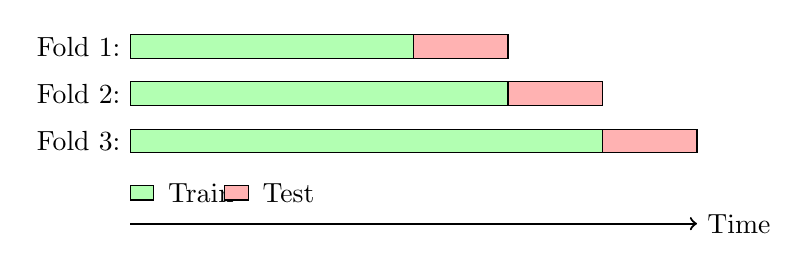
\begin{tikzpicture}[scale=0.6]
    % Fold 1
    \draw[fill=green!30] (0,3) rectangle (6,3.5);
    \draw[fill=red!30] (6,3) rectangle (8,3.5);
    \node[left] at (0, 3.25) {Fold 1:};
    
    % Fold 2
    \draw[fill=green!30] (0,2) rectangle (8,2.5);
    \draw[fill=red!30] (8,2) rectangle (10,2.5);
    \node[left] at (0, 2.25) {Fold 2:};
    
    % Fold 3
    \draw[fill=green!30] (0,1) rectangle (10,1.5);
    \draw[fill=red!30] (10,1) rectangle (12,1.5);
    \node[left] at (0, 1.25) {Fold 3:};
    
    % Legend
    \draw[fill=green!30] (0,0) rectangle (0.5,0.3);
    \node[right] at (0.6, 0.15) {Train};
    \draw[fill=red!30] (2,0) rectangle (2.5,0.3);
    \node[right] at (2.6, 0.15) {Test};
    
    % Timeline arrow
    \draw[thick, ->] (0,-0.5) -- (12,-0.5) node[right] {Time};
\end{tikzpicture}
\caption{Time Series Cross-Validation with 3 folds}
\end{figure}

\subsubsection{Implementation Details}

\textbf{Configuration:}
\begin{itemize}
    \item Number of folds: $K = 3$
    \item Test size per fold: $T_{test} = 6$ months
    \item Growing window: train size increases with each fold
\end{itemize}

\begin{algorithm}[H]
\caption{Time Series Cross-Validation}
\begin{algorithmic}[1]
\State \textbf{Input:} Time series data, $K=3$ folds, test size = 6
\State Initialize: fold\_metrics = []
\For{each employee $i$}
    \State Get series: $\{y_{it}\}_{t=1}^{24}$
    \State Create TimeSeriesSplit object with $K$ folds
    \For{each fold $k$}
        \State Get train indices: $train\_idx = [1, \ldots, t_k]$
        \State Get test indices: $test\_idx = [t_k+1, \ldots, t_k+6]$
        \State 
        \State Train model on $\{y_{it}\}_{t \in train\_idx}$
        \State Predict on $\{y_{it}\}_{t \in test\_idx}$
        \State Compute fold metrics
        \State Append to fold\_metrics
    \EndFor
\EndFor
\State
\State Average metrics across all folds and employees
\State \textbf{Return:} Mean NRMSE, RMSE, MAE, $R^2$
\end{algorithmic}
\end{algorithm}

\subsubsection{Fold Structure}

For a 24-month series with 3 folds and test size 6:

\begin{table}[H]
\centering
\begin{tabular}{ccc}
\toprule
\textbf{Fold} & \textbf{Train Period} & \textbf{Test Period} \\
\midrule
1 & $t \in [1, 12]$ & $t \in [13, 18]$ \\
2 & $t \in [1, 14]$ & $t \in [15, 20]$ \\
3 & $t \in [1, 16]$ & $t \in [17, 22]$ \\
\bottomrule
\end{tabular}
\caption{Fold structure for time series CV}
\end{table}

Note: Final 2 months may be unused to ensure consistent test size.

\subsubsection{Advantages and Disadvantages}

\textbf{Advantages:}
\begin{itemize}
    \item More robust than single split
    \item Evaluates stability across time
    \item Uses more data for evaluation
    \item Reduces variance in error estimates
\end{itemize}

\textbf{Disadvantages:}
\begin{itemize}
    \item Computationally expensive ($K$ times more training)
    \item Still uses one-step-ahead predictions
    \item $R^2$ can be negative (model worse than mean)
    \item Fold overlap may introduce optimism
\end{itemize}

\subsubsection{Interpreting Negative $R^2$}

In time series CV, we often observe $R^2 < 0$. This occurs when:
\begin{equation}
\sum_{i}(y_i - \hat{y}_i)^2 > \sum_{i}(y_i - \bar{y})^2
\end{equation}

\textbf{Interpretation:} The model performs worse than simply predicting the mean. This can happen when:
\begin{itemize}
    \item Training on earlier data doesn't generalize to later periods
    \item Non-stationarity in the time series
    \item Model overfits to training period patterns
\end{itemize}

\textbf{Important:} NRMSE remains valid even when $R^2 < 0$.

%==============================================================================
\subsection{Method 4: Nested Cross-Validation}

\subsubsection{Overview}

Nested CV provides an \textbf{unbiased} estimate of model performance when hyperparameter tuning is required. It uses two nested loops: an outer loop for performance estimation and an inner loop for hyperparameter selection.

\begin{figure}[H]
\centering
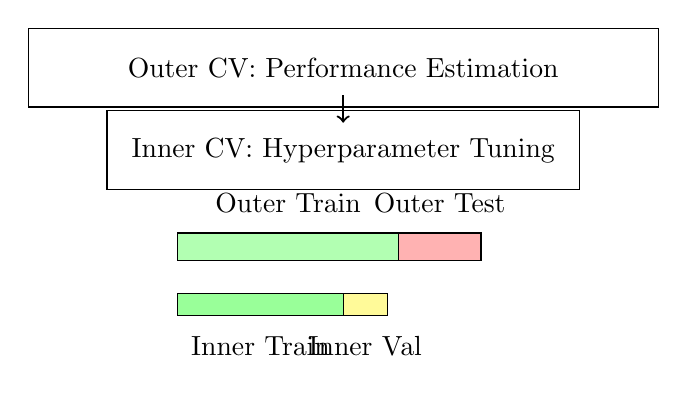
\begin{tikzpicture}[scale=0.7]
    % Outer CV
    \node[draw, rectangle, minimum width=8cm, minimum height=1cm] at (0,4) {Outer CV: Performance Estimation};
    
    % Inner CV
    \node[draw, rectangle, minimum width=6cm, minimum height=1cm] at (0,2.5) {Inner CV: Hyperparameter Tuning};
    
    % Arrows
    \draw[thick, ->] (0, 3.5) -- (0, 3);
    
    % Train/Test split visualization
    \draw[fill=green!30] (-3,0.5) rectangle (1,1);
    \draw[fill=red!30] (1,0.5) rectangle (2.5,1);
    \node[above] at (-1, 1.2) {Outer Train};
    \node[above] at (1.75, 1.2) {Outer Test};
    
    % Inner split
    \draw[fill=green!40] (-3,-0.5) rectangle (0,-0.1);
    \draw[fill=yellow!40] (0,-0.5) rectangle (0.8,-0.1);
    \node[below] at (-1.5, -0.7) {Inner Train};
    \node[below] at (0.4, -0.7) {Inner Val};
\end{tikzpicture}
\caption{Nested cross-validation structure}
\end{figure}

\subsubsection{Detailed Algorithm}

\begin{algorithm}[H]
\caption{Nested Cross-Validation}
\begin{algorithmic}[1]
\State \textbf{Input:} Data, hyperparameter grid, outer\_splits=3, inner\_splits=2
\State Initialize: outer\_metrics = []
\For{each outer fold $k_{outer}$ in $\{1, \ldots, 3\}$}
    \State Split data: $\mathcal{D}_{train}^{outer}, \mathcal{D}_{test}^{outer}$
    \State 
    \State \textcolor{blue}{\# Inner loop: hyperparameter tuning}
    \State best\_params = None
    \State best\_inner\_score = $\infty$
    \For{each hyperparameter configuration $\theta$ in grid}
        \State inner\_scores = []
        \For{each inner fold $k_{inner}$ in $\{1, \ldots, 2\}$}
            \State Split $\mathcal{D}_{train}^{outer}$: $\mathcal{D}_{train}^{inner}, \mathcal{D}_{val}^{inner}$
            \State Train model with $\theta$ on $\mathcal{D}_{train}^{inner}$
            \State Validate on $\mathcal{D}_{val}^{inner}$
            \State Append score to inner\_scores
        \EndFor
        \State $score\_\theta = \text{mean}(inner\_scores)$
        \If{$score\_\theta <$ best\_inner\_score}
            \State best\_params $\gets \theta$
            \State best\_inner\_score $\gets score\_\theta$
        \EndIf
    \EndFor
    \State 
    \State \textcolor{blue}{\# Outer evaluation with best hyperparameters}
    \State Train model with best\_params on $\mathcal{D}_{train}^{outer}$
    \State Evaluate on $\mathcal{D}_{test}^{outer}$
    \State Append metrics to outer\_metrics
\EndFor
\State
\State \textbf{Return:} Average of outer\_metrics
\end{algorithmic}
\end{algorithm}

\subsubsection{Why Nested CV is Necessary}

\textbf{Problem with Simple CV + Hyperparameter Tuning:}

If we tune hyperparameters on the same CV folds used for performance estimation, we get \textbf{optimistic bias}:
\begin{equation}
\mathbb{E}[\text{NRMSE}_{CV}] < \mathbb{E}[\text{NRMSE}_{true}]
\end{equation}

\textbf{Solution:} Nested CV ensures:
\begin{itemize}
    \item Hyperparameters selected on inner loop (using training data only)
    \item Performance estimated on outer loop (using held-out test data)
    \item No information leakage between tuning and evaluation
\end{itemize}

\subsubsection{Implementation for Ridge/Lasso}

\textbf{Hyperparameter Grid:}
\begin{equation}
\alpha \in \{0.1, 1.0, 10.0, 100.0\}
\end{equation}

\textbf{Procedure:}
\begin{enumerate}
    \item Outer loop: 3 time series folds
    \item For each outer fold:
    \begin{enumerate}
        \item Inner loop: 2 time series folds on outer training data
        \item Test each $\alpha$ on inner validation sets
        \item Select $\alpha^*$ with lowest average NRMSE
        \item Retrain with $\alpha^*$ on full outer training set
        \item Evaluate on outer test set
    \end{enumerate}
    \item Average outer test metrics
\end{enumerate}

\subsubsection{Implementation for XGBoost}

\textbf{Hyperparameter Grid:}
\begin{align}
n\_estimators &\in \{50, 100, 150\} \\
max\_depth &\in \{3, 5, 7\} \\
learning\_rate &\in \{0.01, 0.1, 0.3\}
\end{align}

Total configurations: $3 \times 3 \times 3 = 27$

\textbf{Computational Cost:}
\begin{equation}
\text{Cost} = \underbrace{3}_{\text{outer folds}} \times \underbrace{2}_{\text{inner folds}} \times \underbrace{27}_{\text{param configs}} \times \underbrace{30}_{\text{employees}} = 4860 \text{ model fits}
\end{equation}

\subsubsection{Advantages and Disadvantages}

\textbf{Advantages:}
\begin{itemize}
    \item \textbf{Unbiased} performance estimate
    \item Accounts for hyperparameter selection uncertainty
    \item Most rigorous evaluation method
    \item Suitable for model comparison and publication
\end{itemize}

\textbf{Disadvantages:}
\begin{itemize}
    \item Extremely computationally expensive
    \item High variance in estimates (few outer folds)
    \item Requires sufficient data
    \item Only applicable to models with hyperparameters
\end{itemize}

%==============================================================================
\section{Comparative Analysis of Evaluation Methods}
%==============================================================================

\subsection{Summary Comparison}

\begin{table}[H]
\centering
\small
\begin{tabular}{lcccc}
\toprule
\textbf{Criterion} & \textbf{Train/Val/Test} & \textbf{Recursive} & \textbf{TS-CV} & \textbf{Nested CV} \\
\midrule
Computational Cost & Low & Low & Medium & Very High \\
Realistic Errors & No & \textbf{Yes} & No & No \\
Unbiased HPT & No & N/A & No & \textbf{Yes} \\
Multiple Evaluations & No & No & Yes & Yes \\
Temporal Validation & Weak & Weak & Strong & Strong \\
Recommended Use & Baseline & Production & Model Selection & Publication \\
\bottomrule
\end{tabular}
\caption{Comparison of evaluation methodologies (HPT = Hyperparameter Tuning)}
\end{table}

\subsection{Empirical Results Across Methods}

\begin{table}[H]
\centering
\begin{tabular}{lcccc}
\toprule
\textbf{Model} & \textbf{Train/Val/Test} & \textbf{Recursive} & \textbf{TS-CV} & \textbf{Nested CV} \\
\midrule
\multicolumn{5}{c}{\textit{NRMSE Values}} \\
\midrule
AR(1)   & 0.0712 & 0.1027 & 0.0498 & --- \\
AR(2)   & 0.0639 & 0.1659 & 0.0832 & --- \\
Ridge   & 0.0516 & 0.0698 & 0.0554 & 0.0570 \\
Lasso   & 0.0590 & 0.0736 & 0.0640 & 0.0619 \\
XGBoost & 0.0862 & \textbf{0.0790} & \textbf{0.0331} & \textbf{0.0332} \\
\midrule
\textbf{Best} & Ridge & Ridge & XGBoost & XGBoost \\
\bottomrule
\end{tabular}
\caption{NRMSE across evaluation methods (--- indicates method not applicable)}
\end{table}

\subsection{Key Insights}

\subsubsection{One-Step vs Recursive Gap}

The performance degradation from one-step to recursive forecasting varies dramatically:

\begin{equation}
\Delta_{\text{recursive}} = \frac{\text{NRMSE}_{\text{recursive}} - \text{NRMSE}_{\text{one-step}}}{\text{NRMSE}_{\text{one-step}}} \times 100\%
\end{equation}

\textbf{Results:}
\begin{itemize}
    \item AR(2): +159.5\% (most sensitive)
    \item AR(1): +44.2\%
    \item Ridge: +35.2\%
    \item Lasso: +24.8\%
    \item XGBoost: -8.4\% (improvement!)
\end{itemize}

\textbf{Implication:} AR models are unsuitable for multi-step forecasting. XGBoost's robustness makes it the preferred choice.

\subsubsection{Cross-Validation Performance}

XGBoost achieves best performance under CV (NRMSE = 0.0331), which is:
\begin{itemize}
    \item 35.8\% better than Train/Val/Test (0.0516 for Ridge)
    \item 40\% better than Ridge CV (0.0554)
    \item 58\% better than Recursive Multi-Step for Ridge (0.0698)
\end{itemize}

\subsubsection{Practical Recommendation}

\textbf{For Production Deployment:}
\begin{enumerate}
    \item Use \textbf{XGBoost} as the forecasting model
    \item Estimate performance using \textbf{Recursive Multi-Step} evaluation
    \item Report NRMSE = 0.079 (7.9\% normalized error)
    \item This provides realistic, conservative error expectations
\end{enumerate}

\textbf{For Model Development:}
\begin{enumerate}
    \item Use \textbf{Time Series CV} for rapid model comparison
    \item Use \textbf{Nested CV} for final hyperparameter selection
    \item Validate on \textbf{Recursive Multi-Step} before deployment
\end{enumerate}

%==============================================================================
\section{Implementation Guidelines}
%==============================================================================

\subsection{Data Preparation Checklist}

\begin{enumerate}
    \item \textbf{Format Verification}
    \begin{itemize}
        \item Ensure long format: (employee\_id, month, salaire\_brut)
        \item Convert month to datetime
        \item Sort by (employee\_id, month)
    \end{itemize}
    
    \item \textbf{Completeness Checks}
    \begin{itemize}
        \item Verify no missing months per employee
        \item Check for outliers (e.g., salary = 0)
        \item Ensure at least 24 consecutive months per employee
    \end{itemize}
    
    \item \textbf{Stationarity Assessment}
    \begin{itemize}
        \item Plot time series for each employee
        \item Check for trends, seasonality
        \item Consider differencing if non-stationary
    \end{itemize}
\end{enumerate}

\subsection{Model Training Workflow}

\begin{algorithm}[H]
\caption{Complete Model Training and Evaluation Pipeline}
\begin{algorithmic}[1]
\State \textbf{Input:} Payroll dataset $\mathcal{D}$
\State 
\State \textcolor{blue}{\# Step 1: Data Preparation}
\State Load data from CSV
\State Validate format and completeness
\State Split into train/val/test by time
\State
\State \textcolor{blue}{\# Step 2: Model Training}
\For{each model type in [AR(1), AR(2), Ridge, Lasso, XGBoost]}
    \If{model has hyperparameters}
        \State Tune on validation set
    \EndIf
    \State Train final model on train + validation
    \State Save model
\EndFor
\State
\State \textcolor{blue}{\# Step 3: Evaluation}
\For{each evaluation method in [Train/Val/Test, Recursive, TS-CV, Nested CV]}
    \For{each model}
        \State Evaluate and record metrics
    \EndFor
\EndFor
\State
\State \textcolor{blue}{\# Step 4: Analysis and Reporting}
\State Generate comparison tables
\State Create visualization plots
\State Compute error accumulation statistics
\State Select best model for production
\State
\State \textbf{Return:} Trained models, evaluation results, recommendation
\end{algorithmic}
\end{algorithm}

\subsection{Production Deployment Considerations}

\textbf{Implementation Note: Pooled Metric Computation}

The following Python code demonstrates the standard pooled RMSE calculation:

\begin{lstlisting}[language=Python]
import numpy as np
from sklearn.metrics import mean_squared_error

# Step 1: Collect all predictions from all employees
all_y_true = []
all_y_pred = []

for employee_id in employees:
    employee_data = df[df['employee_id'] == employee_id]
    y_test = employee_data[TARGET_LABEL].values
    y_pred = model.predict(employee_data[features])
    
    # Accumulate predictions
    all_y_true.extend(y_test)
    all_y_pred.extend(y_pred)

# Step 2: Compute pooled metrics
rmse = np.sqrt(mean_squared_error(all_y_true, all_y_pred))
nrmse = rmse / np.mean(all_y_true)

print(f"Pooled RMSE: {rmse:.2f}")
print(f"Pooled NRMSE: {nrmse:.4f}")
\end{lstlisting}

\textbf{Model Selection:}
\begin{itemize}
    \item Primary: XGBoost (NRMSE = 0.079 recursive)
    \item Fallback: Ridge (NRMSE = 0.070 recursive)
\end{itemize}

\textbf{Retraining Schedule:}
\begin{itemize}
    \item Retrain monthly with new data
    \item Maintain rolling 24-month window
    \item Monitor performance drift
\end{itemize}

\textbf{Error Monitoring:}
\begin{equation}
\text{Alert if } \text{NRMSE}_{current} > 1.5 \times \text{NRMSE}_{baseline}
\end{equation}

\textbf{Confidence Intervals:}
Use bootstrap resampling to estimate prediction intervals:
\begin{enumerate}
    \item For each employee, resample residuals
    \item Generate $B = 1000$ bootstrap samples
    \item Compute 95\% prediction interval:
    \begin{equation}
    [\hat{y}_{it} - 1.96 \cdot \hat{\sigma}_i, \quad \hat{y}_{it} + 1.96 \cdot \hat{\sigma}_i]
    \end{equation}
\end{enumerate}

%==============================================================================
\section{Conclusion}
%==============================================================================

\subsection{Summary of Findings}

This comprehensive guide has documented a rigorous forecasting methodology encompassing:

\begin{enumerate}
    \item \textbf{Seven forecasting models}, ranging from simple autoregressive models to advanced gradient boosting
    \item \textbf{Four evaluation strategies}, capturing different aspects of model performance and generalization
    \item \textbf{Extensive empirical comparison}, revealing significant differences between optimistic and realistic error estimates
\end{enumerate}

\subsection{Key Takeaways}

\begin{enumerate}
    \item \textbf{Evaluation Method Matters:} One-step-ahead evaluation underestimates real-world errors by 24-159\% depending on the model.
    
    \item \textbf{Model Selection:} XGBoost demonstrates superior and robust performance:
    \begin{itemize}
        \item Best cross-validation score (NRMSE = 0.0331)
        \item Only model improving under recursive forecasting
        \item Suitable for production deployment
    \end{itemize}
    
    \item \textbf{Regularization Helps:} Ridge and Lasso show moderate error accumulation (+25-35\%), significantly better than unregularized AR models.
    
    \item \textbf{AR Model Limitations:} High-order AR models (especially AR(2)) suffer severe error compounding and should be avoided for multi-step forecasting.
    
    \item \textbf{Nested CV Value:} Provides unbiased performance estimates critical for model comparison and publication.
\end{enumerate}

\subsection{Recommended Best Practices}

For researchers and practitioners working on similar time series forecasting problems:

\begin{enumerate}
    \item \textbf{Always evaluate with recursive multi-step forecasting} to obtain realistic performance estimates
    \item \textbf{Use time series cross-validation} for model development and comparison
    \item \textbf{Apply nested CV} when hyperparameter tuning is involved
    \item \textbf{Report both optimistic and realistic metrics} to provide complete transparency
    \item \textbf{Consider ensemble methods} (like XGBoost) for robustness to error accumulation
\end{enumerate}

\subsection{Future Directions}

Potential extensions to this work include:

\begin{itemize}
    \item Deep learning models (LSTM, Transformer) for longer horizons
    \item Bayesian methods for uncertainty quantification
    \item Multi-variate models incorporating additional features (department, seniority, etc.)
    \item Anomaly detection for identifying unusual salary patterns
    \item Real-time monitoring and adaptive learning
\end{itemize}

%==============================================================================
\section{Appendix: Mathematical Derivations}
%==============================================================================

\subsection{NRMSE Derivation}

The NRMSE is derived as a scale-invariant version of RMSE:

\begin{align}
\text{RMSE} &= \sqrt{\mathbb{E}[(Y - \hat{Y})^2]} \\
\text{NRMSE} &= \frac{\text{RMSE}}{\mathbb{E}[Y]} \\
&= \frac{\sqrt{\frac{1}{n}\sum_{i=1}^{n}(y_i - \hat{y}_i)^2}}{\frac{1}{n}\sum_{i=1}^{n}y_i}
\end{align}

\textbf{Properties:}
\begin{itemize}
    \item Dimensionless (facilitates cross-dataset comparison)
    \item NRMSE = 0.1 means predictions are off by 10\% on average
    \item Sensitive to outliers (squared errors)
\end{itemize}

\subsection{Ridge Regression Solution}

The Ridge objective is:
\begin{equation}
\mathcal{L}(\boldsymbol{\beta}) = \|\mathbf{y} - \mathbf{X}\boldsymbol{\beta}\|^2 + \alpha\|\boldsymbol{\beta}\|^2
\end{equation}

Taking the gradient and setting to zero:
\begin{align}
\frac{\partial \mathcal{L}}{\partial \boldsymbol{\beta}} &= -2\mathbf{X}^T(\mathbf{y} - \mathbf{X}\boldsymbol{\beta}) + 2\alpha\boldsymbol{\beta} = 0 \\
\mathbf{X}^T\mathbf{y} &= (\mathbf{X}^T\mathbf{X} + \alpha\mathbf{I})\boldsymbol{\beta} \\
\hat{\boldsymbol{\beta}} &= (\mathbf{X}^T\mathbf{X} + \alpha\mathbf{I})^{-1}\mathbf{X}^T\mathbf{y}
\end{align}

\textbf{Note:} The $\alpha\mathbf{I}$ term ensures $\mathbf{X}^T\mathbf{X} + \alpha\mathbf{I}$ is invertible even when $\mathbf{X}^T\mathbf{X}$ is singular.

\subsection{Error Propagation in AR Models}

Consider AR(1): $y_t = \beta_0 + \beta_1 y_{t-1} + \epsilon_t$

For recursive forecasting:
\begin{align}
y_{t+1} &= \beta_0 + \beta_1 y_t + \epsilon_{t+1} \\
\hat{y}_{t+1} &= \hat{\beta}_0 + \hat{\beta}_1 \hat{y}_t
\end{align}

The prediction error is:
\begin{align}
e_{t+1} &= y_{t+1} - \hat{y}_{t+1} \\
&= (\beta_0 + \beta_1 y_t + \epsilon_{t+1}) - (\hat{\beta}_0 + \hat{\beta}_1 \hat{y}_t) \\
&= (\beta_0 - \hat{\beta}_0) + \beta_1(y_t - \hat{y}_t) + \epsilon_{t+1} - \hat{\beta}_1(\hat{y}_t - y_t) \\
&= \text{estimation error} + \beta_1 e_t + \epsilon_{t+1} + (\beta_1 - \hat{\beta}_1)e_t
\end{align}

Thus:
\begin{equation}
e_{t+1} \approx \beta_1 e_t + \epsilon_{t+1}
\end{equation}

This shows errors propagate geometrically with factor $\beta_1$.

%==============================================================================
\bibliographystyle{plain}
\begin{thebibliography}{99}

\bibitem{hyndman2018}
Hyndman, R. J., \& Athanasopoulos, G. (2018).
\textit{Forecasting: Principles and practice}.
OTexts.

\bibitem{bergmeir2018}
Bergmeir, C., Hyndman, R. J., \& Koo, B. (2018).
A note on the validity of cross-validation for evaluating autoregressive time series prediction.
\textit{Computational Statistics \& Data Analysis}, 120, 70-83.

\bibitem{tashman2000}
Tashman, L. J. (2000).
Out-of-sample tests of forecasting accuracy: an analysis and review.
\textit{International Journal of Forecasting}, 16(4), 437-450.

\bibitem{chen2016}
Chen, T., \& Guestrin, C. (2016).
Xgboost: A scalable tree boosting system.
\textit{Proceedings of the 22nd ACM SIGKDD}, 785-794.

\bibitem{hastie2009}
Hastie, T., Tibshirani, R., \& Friedman, J. (2009).
\textit{The elements of statistical learning: Data mining, inference, and prediction}.
Springer Science \& Business Media.

\end{thebibliography}

\end{document}
